\documentclass[handout]{beamer}
\title[] % (optional, only for long titles)
{Algorithmic Verification of Channel Machines Using Small Models}
\author[J, Sharyari | \emph{sharyari@gmail.com}] {Jonathan Sharyari}
\usetheme[numbers]{Uppsala}
\subject{Computer Science}


\usepackage{tikz}
\usetikzlibrary{arrows}
\usetikzlibrary{automata,positioning,shapes}

\newcommand{\petersonone}[1][]{
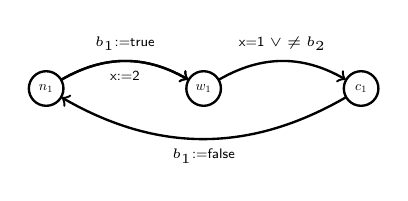
\begin{tikzpicture} [->,auto,node distance=2.0cm,line width=0.3mm]

  \node[state] (1) [scale=0.5]{$n_1$};
  \node[state] (2) [right of=1, scale=0.5] {$w_1$};
  \node[state] (3) [right of=2, scale=0.5] {$c_1$};

  \path[every node/.style={font=\sffamily\tiny}]
    (1) edge [bend left] node [above] {$b_1$:=true} (2)
    (1) edge [bend left] node [below] {x:=2} (2)
    (2) edge [bend left] node [above] {x=1 $\vee$ $\neq$ $b_2$} (3)
    (3) edge [bend left] node [below] {$b_1$:=false} (1);

\end{tikzpicture}
}




\newcommand{\petersontwo}[1][]{
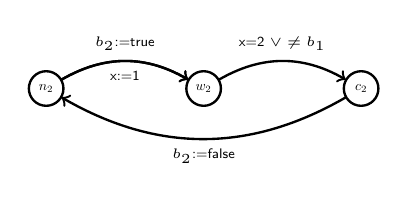
\begin{tikzpicture} [->,auto,node distance=2.0cm,line width=0.3mm]

  \node[state] (1) [scale=0.5]{$n_2$};
  \node[state] (2) [right of=1, scale=0.5] {$w_2$};
  \node[state] (3) [right of=2, scale=0.5] {$c_2$};

  \path[every node/.style={font=\sffamily\tiny}]
    (1) edge [bend left] node [above] {$b_2$:=true} (2)
    (1) edge [bend left] node [below] {x:=1} (2)
    (2) edge [bend left] node [above] {x=2 $\vee$ $\neq$ $b_1$} (3)
    (3) edge [bend left] node [below] {$b_2$:=false} (1);

\end{tikzpicture}
}



\newcommand{\petersonboth}[1][]{
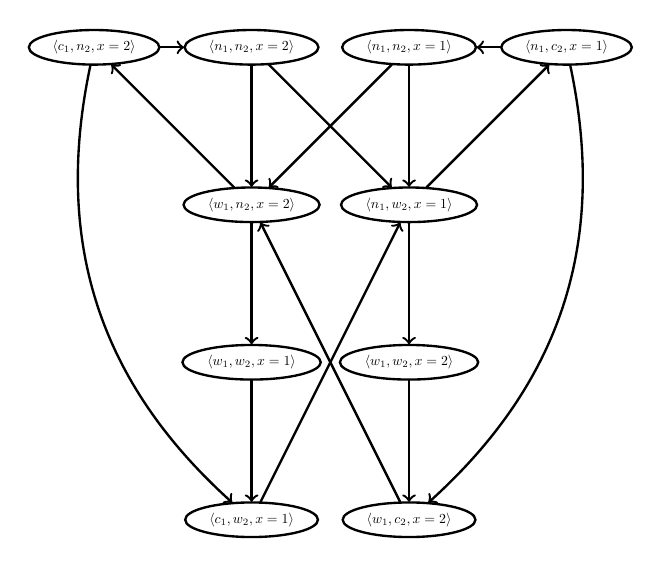
\begin{tikzpicture} [->,auto,node distance=2.0cm,line width=0.3mm]

  \node[state] (1) [ellipse,scale=0.5]{$\langle c_1,n_2,x=2\rangle$};
  \node[state] (2) [ellipse,right of=1, scale=0.5] {$\langle n_1,n_2,x=2\rangle$};
  \node[state] (3) [ellipse,right of=2, scale=0.5] {$\langle n_1,n_2,x=1\rangle$};
  \node[state] (4) [ellipse,right of=3,scale=0.5]{$\langle n_1,c_2, x=1\rangle$};
  \node[state] (5) [ellipse,below of=2, scale=0.5] {$\langle w_1,n_2,x=2\rangle$};
  \node[state] (6) [ellipse,below of=5, scale=0.5] {$\langle w_1,w_2,x=1\rangle$};
  \node[state] (7) [ellipse,below of=6, scale=0.5]{$\langle c_1, w_2,x=1\rangle$};
  \node[state] (8) [ellipse,below of=3, scale=0.5] {$\langle n_1,w_2,x=1\rangle$};
  \node[state] (9) [ellipse,below of=8, scale=0.5] {$\langle w_1,w_2, x=2\rangle$};
  \node[state] (10) [ellipse,below of=9, scale=0.5] {$\langle w_1,c_2,x=2\rangle$};


  \path[every node/.style={font=\sffamily\tiny}]
    (1) edge node [above] {} (2)
        edge [bend right] node [below] {} (7)
    (2) edge  node [below] {} (5)
        edge  node [below] {} (8)
    (3) edge node [above] {} (5)
        edge node [below] {} (8)
    (4) edge node [below] {} (3)
        edge [bend left] node [below] {} (10)
    (5) edge node [below] {} (6)
	edge node [below] {} (1)
    (6) edge node [below] {} (7)
    (7) edge node [below] {} (8)
    (8) edge node [below] {} (9)
	edge node [below] {} (4)
    (9) edge node [below] {} (10)
    (10) edge node [below] {} (5);



\end{tikzpicture}
}

\newcommand{\burns}[1][]{
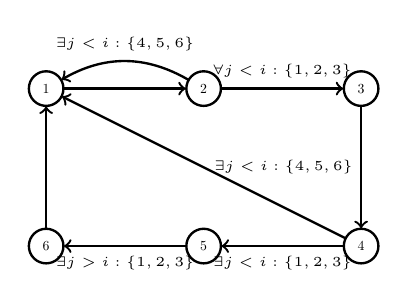
\begin{tikzpicture} [->,auto,node distance=2.0cm,line width=0.3mm]

  \node[state] (1) [scale=0.5]{$1$};
  \node[state] (2) [right of=1, scale=0.5] {$2$};
  \node[state] (3) [right of=2, scale=0.5] {$3$};
  \node[state] (4) [below of=3, scale=0.5] {$4$};
  \node[state] (5) [left of=4, scale=0.5] {$5$};
  \node[state] (6) [left of=5, scale=0.5]{$6$};

  \path[every node/.style={font=\sffamily\tiny}]
    (1) edge node [above] {} (2)
    (2) edge [bend right] node [above] {$\exists j<i: \{4,5,6\}$} (1)
     edge node [above] {$\forall j<i:\{1,2,3\}$} (3)
    (3) edge node [below] {} (4)
    (4) edge node [right] {$\exists j<i: \{4,5,6\}$} (1)
    (4) edge node [below] {$\exists j<i: \{1,2,3\}$} (5)
    (5) edge node [below] {$\exists j>i: \{1,2,3\}$} (6)
    (6) edge node [above] {} (1);
\end{tikzpicture}
}


\newcommand{\abpobserver}[1][]{
\begin{tikzpicture} [->,auto,node distance=3.0cm,line width=0.3mm]

%\begin{tikzpicture}[->,>=stealth',shorten >=1pt,auto,node distance=3cm,
%  thick,main node/.style={circle,fill=blue!20,draw,font=\sffamily\Large\bfseries}]

  \node[scale=0.5, state] (1) {$o_1$};
  \node[scale=0.5,state,accepting] (3) [right of=1] {$o_2$};
  \node[scale=0.5,state] (2) [right of=2] {$o_3$};

  \path[every node/.style={font=\sffamily\tiny}]
    (1) edge [bend left] node [above] {Snd} (2)
        edge node [above] {Rcv} (3)
    (2) edge [bend left] node [below] {Rcv} (1)
        edge node [above] {Snd} (3);
\end{tikzpicture}
}

\newcommand{\abpsender}[1][]{
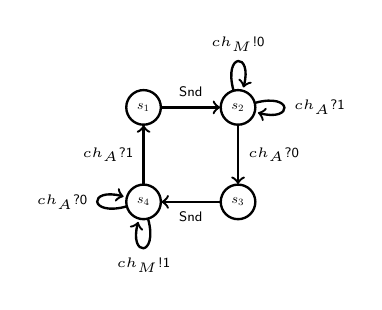
\begin{tikzpicture} [->,auto,node distance=2.4cm,line width=0.3mm]
  \node[scale=0.5,state] (1) {$s_1$};
  \node[scale=0.5,state] (2) [right of=1] {$s_2$};
  \node[scale=0.5,state] (3) [below of=2] {$s_3$};
  \node[scale=0.5,state] (4) [left of=3] {$s_4$};

  \path[every node/.style={font=\sffamily\tiny}]
    (1) edge node [above] {Snd} (2)
    (2) edge node [right] {$ch_A$?0} (3)
        edge [loop right] node {$ch_A$?1} (2)
        edge [loop above] node {$ch_M$!0} (2)
    (3) edge node [below] {Snd} (4)
    (4) edge node [left] {$ch_A$?1} (1)
        edge [loop left] node {$ch_A$?0} (4)
        edge [loop below] node {$ch_M$!1} (4);
\end{tikzpicture}
}

\newcommand{\abpreceiver}[1][]{
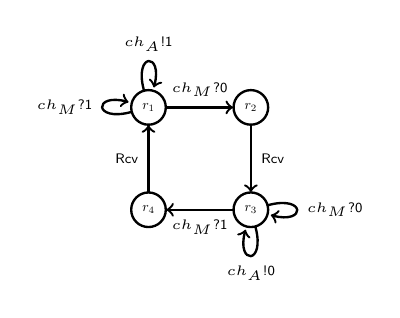
\begin{tikzpicture} [->,auto,node distance=2.6cm,line width=0.3mm]

  \node[scale=0.5,state] (1) {$r_1$};
  \node[scale=0.5,state] (2) [right of=1] {$r_2$};
  \node[scale=0.5,state] (3) [below of=2] {$r_3$};
  \node[scale=0.5,state] (4) [left of=3] {$r_4$};

  \path[every node/.style={font=\sffamily\tiny}]
    (1) edge node [above] {$ch_M$?0} (2)
        edge [loop left] node {$ch_M$?1} (1)
        edge [loop above] node {$ch_A$!1} (1)
    (2) edge node [right] {Rcv} (3)
    (3) edge node [below] {$ch_M$?1} (4)
        edge [loop right] node {$ch_M$?0} (3)
        edge [loop below] node {$ch_A$!0} (3)
    (4) edge node [left] {Rcv} (1);

\end{tikzpicture}
}


\newcommand{\abstraction}[1][]{
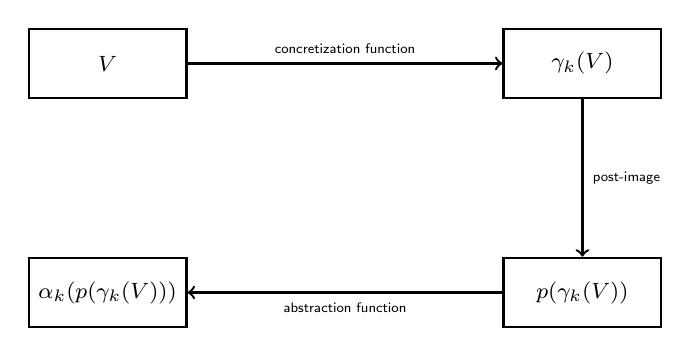
\begin{tikzpicture} [->,auto,node distance=2cm and 4cm,line width=0.3mm, font=\footnotesize]

  \node[state] (1) [rectangle, minimum width=2cm] {$V$};
  \node[state] (2) [rectangle, minimum width=2cm,right=of 1] {$\gamma_k(V)$};
  \node[state] (3) [rectangle, minimum width=2cm,below=of 2] {$p(\gamma_k(V))$};
  \node[state] (4) [rectangle, minimum width=2cm,left=of 3] {$\alpha_k(p(\gamma_k(V)))$};

  \path[every node/.style={font=\sffamily\tiny}]
    (1) edge node [above] {concretization function} (2)
    (2) edge node [right] {post-image} (3)
    (3) edge node [below] {abstraction function} (4);

\end{tikzpicture}
}


\newcommand{\freachability}[1][]{
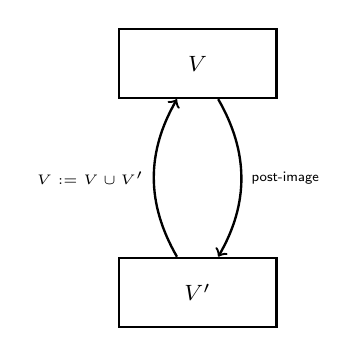
\begin{tikzpicture} [->,auto,node distance=2cm and 4cm,line width=0.3mm, font=\footnotesize]

  \node[state] (1) [rectangle, minimum width=2cm] {$V$};
  \node[state] (2) [rectangle, minimum width=2cm,below=of 1] {$V'$};

  \path[every node/.style={font=\sffamily\tiny}]
    (1) edge [bend left] node [right] {post-image} (2)
    (2) edge [bend left] node [left] {$V := V \cup V'$} (1);
\end{tikzpicture}
}

\date[2014-09-09] % appears in the bottom of the sidebar
{September $9^{th}$, 2014}
\institute[Dept. of Information Technology] % appears in the footline
{
  Department of Information Technology\\
  Uppsala University \\ \vspace{10pt}
  Supervisor: Parosh Abdulla \\
  Reviewer: Mohamed Faouzi Atig
}
\usepackage{float}
\newfloat{algorithm}{t}{lop}
%\usepackage{subfigure}
\usepackage{subcaption}
\usepackage{algpseudocode}
\usepackage{biblatex}
\usepackage[usenames,svgnames]{xcolor}

%\addbibresource{references.bib}
\algtext*{EndWhile}% Remove "end while" text
\algtext*{EndIf}% Remove "end if" text
\algtext*{EndFor}% Remove "end if" text
\begin{document}
\begin{frame}[plain]
  \titlepage
\end{frame}

\begin{frame}
  \tableofcontents

\end{frame}

\section{General Verification}
\subsection*{1}
\begin{frame}
  \frametitle{Verification}
  \begin{itemize}
  \item
    Verification is the “process of evaluating software to determine whether the products of a given development phase satisfy the conditions imposed at the start of that phase”\cite{ordbok}
  \item
    Model checking is the task of automatically verifying the correctness of a program, with regard to its specification.
  \end{itemize}
\end{frame}

\subsection*{1}
\begin{frame}
  \frametitle{Peterson's Mutual Exclusion -- Pseudo Code}

  \begin{algorithmic}
    \small
    \While{true}
    \State $\langle b_1$:= true, $x$:=true$\rangle$;
    \State \textbf{await} ($x$=1 $\vee$ $\neq$ $b_2$);
    \State \textsc{critical section}
    \State $b_1$ := false
    \EndWhile
  \end{algorithmic}

  % This slide should have a simple example, for example two counters or something, to illustrate how graphs are ``searched''.
  % Introduce the concept of a ``bad state''
  % Bakery algorithm, forward reachability, backward reachability...

\end{frame}

\subsection*{1}
\begin{frame}
  \begin{example}[Program Graphs]
    \frametitle{Petersons's Mutual Exclusion -- Program Graph}
    \petersonone

    \petersontwo
  \end{example}
  \begin{itemize}
  \item
    $\langle$ $c_1$,$c_2$ $\rangle$ is a \emph{bad global state}
  \end{itemize}

\end{frame}

\subsection*{1}
\begin{frame}
  \frametitle{Peterson's Mutual Exclusion -- Transition System}
  \begin{example}[Transition System]
    \petersonboth
  \end{example}
  % Mention that there are several ways to check for this. This is a case of forward reachability...
\end{frame}


\section{All for the Price of Few}
\subsection*{1}
\begin{frame}
  \frametitle{All for the Price of Few}
  \begin{itemize}
  \item Builds upon work by Parosh Abdulla, Fr\'ed\'eric Haziza and Luk\'a\v{s} Hol\'ic, \emph{All for the Price of Few}, 2013
  \item Parameterized Systems
  \item Small models
  \item View abstraction
    % The point of this slide is to present their paper, mention some concepts that I'm going to explain and to explain, that I will explain them in the context of their work, as it is less messy
  \end{itemize}
\end{frame}

\subsection*{1}
\subsection{Parameterized Systems}
\begin{frame}
  \frametitle{Parameterized Systems}
  \begin{itemize}
  \item
    The size of the system is a parameter of the system
  \item
    Results in the verification of an infinite system % One for each size of the system
  \item
    Example: unbounded number of participents, unbounded integers, unbounded channels
    % The point of this slide is to give an idea of why this is a problem, and how this problem surfaces.
    % If instead of the bakery, we would have a protocol with more actors...
  \end{itemize}
\end{frame}

\subsection*{1}
\begin{frame}
  \frametitle{Parameterized Systems -- Burns' Protocol}
  \begin{figure}
    \begin{example}[Burns' Protocol]
      \begin{subfigure}[b]{0.49\textwidth}
        \begin{algorithmic}
          \footnotesize
          \State flags[i] :=0;
          \If{$\exists j<i: flag[i] = 1$} \State \textbf{goto} 1;
          \EndIf
          \State flags[i] :=1;
          \If {$\exists j<i: i: flag[i] = 1$} \State \textbf{goto} 1;
          \EndIf
          \State \textbf{await} $\forall$ j$>$i: flag[j] $\neq$ 1;
          \State flag[i] :=0; \textbf{goto} 1;
        \end{algorithmic}
      \end{subfigure}
      \begin{subfigure}[b]{0.49\textwidth}
        \burns
      \end{subfigure}
    \end{example}
  \end{figure}
\end{frame}


\subsection{Small Models}
\begin{frame}
  \frametitle{Small Models}
  \begin{itemize}
  \item
    In some cases, a ''small'' model of a system may exhibit all the relevant behaviour larger systems. % This is not always possible!
  \item
    It suffices to prove the correctness of a small model
    % The point of this slide is to give an intuitive feeling on how to solve the problem
  \end{itemize}
\end{frame}

\subsection{View Abstraction}
\begin{frame}
  \frametitle{View Abstraction} % mention ``Abstract interpretation''
  \begin{exampleblock}{}
    \abstraction
  \end{exampleblock}
\end{frame}

\subsection*{1}
\begin{frame}
\frametitle{View Abstraction -- Example}
\begin{itemize}
\item
Abstraction function $\alpha$: The \emph{subwords} of configurations
\begin{example}[Abstraction]
  $\alpha_2$(\{1,2,3\}) = \{\{1,2\},\{2,3\},\{1,3\},\{1\},\{2\},\{3\}\}
\end{example}
\item
Concretization function $\gamma$: The ''inverse'' of the abstraction function
\begin{example}[Concretization]
  $\gamma_3$(\{\{1,2\},\{2,3\}, \{1,3\}, \{1\}, \{2\}, \{3\}\}) = \{1,2,3\}
\end{example}
\end{itemize}
\end{frame}
\subsection{Verification Algorithm}
\begin{frame}
  \frametitle{Verification algorithm} % mention ``Abstract interpretation''
  \footnotesize
  \begin{algorithmic}[1]
    \While{\texttt{$True$}}
    \If {$\mathcal{R}_k$ $\cap$ $Bad$ $\neq$ $\emptyset$} \Comment{True if unsafe}
    \State return Unsafe
    \EndIf
    \State V := $\mu X.\alpha_k(I)$ $\cup$ $Apost_k(X)$ \Comment{fixpoint overapproximation}
    \If {$\gamma_k(V)$ $\cap$ $Bad$ = $\emptyset$} \Comment{True if safe}
    \State return Safe
    \EndIf
    \State k := k+1 \Comment{Safe but not a small model}
    \EndWhile
  \end{algorithmic}
\end{frame}

\section{Objective}
\subsection*{1}
\begin{frame}
  \frametitle{Goal}
  \begin{itemize}
  \item
    Adapting the verification method to verify \emph{channel systems}
  \item
    Implementing the verification method
  \end{itemize}
\end{frame}

\begin{frame}
  \tableofcontents
\end{frame}


\section{Method}
\subsection{Channel Systems}
\begin{frame}
  \frametitle{Channel Systems}
  \begin{itemize}
  \item
    A channel system is a system that relies on channels for its operation, e.g. communication protocols
  \item
    If channels are unbounded, the model checking of such protocols corresponds to searching an infinite graph
  \end{itemize}
\end{frame}

\subsection*{1}
\begin{frame}
  \begin{example}[ABP Program Graphs]
    \frametitle{Alternating Bit Protocol -- Program Graphs}
    \begin{figure}
      \begin{subfigure}[b]{0.49\textwidth}
        \abpsender
        \caption{\tiny ABP sender}
      \end{subfigure}
      \begin{subfigure}[b]{0.49\textwidth}
        \abpreceiver
        \caption{\tiny ABP receiver}
      \end{subfigure}
      \begin{subfigure}[b]{\textwidth}
        \center
        \abpobserver
        \caption{\tiny ABP observer}
      \end{subfigure}
    \end{figure}
  \end{example}
\end{frame}

\subsection{Transition System}
\begin{frame}
  \frametitle{Channel Transition System}
  \begin{itemize}
  \item
    Tuples $\langle S, \xi\rangle$, where $S$ is a global state, and $\xi$ is the \emph{evaluation} of channel states.
  \item
    Alternating bit protocol: $\langle [s, r, o], [ch_M, ch_A]\rangle$
  \end{itemize}
\end{frame}

\subsection{$\alpha$ and $\gamma$}
\begin{frame}
  \frametitle{View Abstraction} % mention ``Abstract interpretation''
  \begin{exampleblock}{}
    \abstraction
  \end{exampleblock}
\end{frame}

\subsection*{1}
\begin{frame}
  \frametitle{Abstraction Function}
  \begin{itemize}
  \item
    Creates views of size $k$ from configurations of size $k+1$
  \item
    The cross product of the subwords of all channels.

    \begin{example}[$\alpha$ for ABP with $k=2$]

    $\langle S, [110,0]\rangle$ $\in$ $\gamma_{k+1}(V) \Rightarrow$

    \{$\langle S, [11, 0]\rangle$, $\langle S, [11, \varepsilon]\rangle$, $\langle S, [10, 0]\rangle$, $\langle S, [10, \varepsilon]\rangle$, $\langle S, [1, 0]\rangle$, $\langle S, [1,\varepsilon ]\rangle$, $\langle S,[0,0]\rangle$, $\langle S, [0,\varepsilon]\rangle$, $\langle S, [\varepsilon, 0]\rangle$, $\langle S, [\varepsilon, \varepsilon]\rangle$\} $\subseteq$ $V$

    \end{example}
  \end{itemize}
\end{frame}

\subsection*{1}
\begin{frame}
  \frametitle{Concretization function}
  \begin{itemize}
  \item
    Creates configurations of size $k+1$ from views of size $k$
  \item
    The ''inverse'' of the abstraction function

    \begin{example}[$\gamma$ for ABP with $k=2$]


    \{$\langle S, [11, 0]\rangle$, $\langle S, [11, \varepsilon]\rangle$, $\langle S, [10, 0]\rangle$, $\langle S, [10, \varepsilon]\rangle$, $\langle S, [1, 0]\rangle$, $\langle S, [1,\varepsilon ]\rangle$, $\langle S,[0,0]\rangle$, $\langle S, [0,\varepsilon]\rangle$, $\langle S, [\varepsilon, 0]\rangle$, $\langle S, [\varepsilon, \varepsilon]\rangle$\} $\subseteq$ $V$

  $\Rightarrow$ \{

${\color{red}\langle S, [110,0]\rangle}$,
  $\langle S, [110,\varepsilon]\rangle$,
$\langle S, [111,0]\rangle$,
$\langle S, [111,\varepsilon]\rangle\}$
$\in$ $\gamma_{k+1}(V)$
    \end{example}
  \end{itemize}
\end{frame}

\begin{frame}
  \frametitle{Concretization function}
  \begin{itemize}
  \item
    Creates configurations of size $k+1$ from views of size $k$
  \item
    The ''inverse'' of the abstraction function

    \begin{example}[$\gamma$ for ABP with $k=2$]

    \{
    $\langle S, [11, 0]\rangle$,
    {\color{red}$\langle S, [11, \varepsilon]\rangle$},
    $\langle S, [10, 0]\rangle$,
    {\color{red}$\langle S, [10, \varepsilon]\rangle$},
    $\langle S, [1, 0]\rangle$,
    {\color{red}$\langle S, [1,\varepsilon ]\rangle$},
    $\langle S,[0,0]\rangle$,
    {\color{red}$\langle S, [0,\varepsilon]\rangle$},
    $\langle S, [\varepsilon, 0]\rangle$,
    {\color{red}$\langle S, [\varepsilon, \varepsilon]\rangle$}
    \} $\subseteq$ $V$

    $\Rightarrow$

    \{
    $\langle S, [110,0]\rangle$,
    {\color{red}$\langle S, [110,\varepsilon]\rangle$},
    $\langle S, [111,0]\rangle$,
    $\langle S, [111,\varepsilon]\rangle\}$
    $\in$ $\gamma_{k+1}(V)$
    \end{example}
  \end{itemize}
\end{frame}


\begin{frame}
  \frametitle{Concretization function}
  \begin{itemize}
  \item
    Creates configurations of size $k+1$ from views of size $k$
  \item
    The ''inverse'' of the abstraction function

    \begin{example}[$\gamma$ for ABP with $k=2$]

    \{
    {\color{red}$\langle S, [11, 0]\rangle$},
    {\color{red}$\langle S, [11, \varepsilon]\rangle$},
    $\langle S, [10, 0]\rangle$,
    $\langle S, [10, \varepsilon]\rangle$,
    {\color{red}$\langle S, [1, 0]\rangle$},
    {\color{red}$\langle S, [1,\varepsilon ]\rangle$},
    $\langle S,[0,0]\rangle$,
    $\langle S, [0,\varepsilon]\rangle$,
    {\color{red}$\langle S, [\varepsilon, 0]\rangle$},
    {\color{red}$\langle S, [\varepsilon, \varepsilon]\rangle$}
    \} $\subseteq$ $V$

    $\Rightarrow$

    \{$
    \langle S, [110,0]\rangle$,
    $\langle S, [110,\varepsilon]\rangle$,
    {\color{red}$\langle S, [111,0]\rangle$},
    $\langle S, [111,\varepsilon]\rangle\}$
    $\in$ $\gamma_{k+1}(V)$
    \end{example}
  \end{itemize}
\end{frame}

\begin{frame}
  \frametitle{Concretization function}
  \begin{itemize}
  \item
    Creates configurations of size $k+1$ from views of size $k$
  \item
    The ''inverse'' of the abstraction function

    \begin{example}[$\gamma$ for ABP with $k=2$]

    \{
    $\langle S, [11, 0]\rangle$,
    {\color{red}$\langle S, [11, \varepsilon]\rangle$},
    $\langle S, [10, 0]\rangle$,
    $\langle S, [10, \varepsilon]\rangle$,
    $\langle S, [1, 0]\rangle$,
    {\color{red}$\langle S, [1,\varepsilon ]\rangle$},
    $\langle S,[0,0]\rangle$,
    $\langle S, [0,\varepsilon]\rangle$,
    $\langle S, [\varepsilon, 0]\rangle$,
    {\color{red}$\langle S, [\varepsilon, \varepsilon]\rangle$}
    \} $\subseteq$ $V$

    $\Rightarrow$

    \{
    $\langle S, [110,0]\rangle$,
    $\langle S, [110,\varepsilon]\rangle$,
    $\langle S, [111,0]\rangle$,
    {\color{red}$\langle S, [111,\varepsilon]\rangle\}$}
    $\in$ $\gamma_{k+1}(V)$
    \end{example}
  \end{itemize}
\end{frame}


\section{Results}
\begin{frame}
  \frametitle{Statistics}
  \begin{table}
    \centering
    \tiny

    \makebox[\linewidth]{
      \begin{tabular}{| c || c | c | c | c | c || c | c | c || c | c | }
        \hline & \multicolumn{5}{c||}{} & \multicolumn{3}{c||}{\textbf{Backward}} & \multicolumn{2}{c|}{\textbf{MPass}} \\
        \cline {2-11} & \textbf{k} & \textbf{size(V)} & \textbf{Result} & \textbf{Time} & \textbf{Mem} & \textbf{Size V} & \textbf{Result} & \textbf{Time} & \textbf{Result} & \textbf{Time} \\
        \hline
        \textsc{abp} & 2 & 108 & Safe & 0.00s & 1MB & 56 & Safe &  0.01s & Safe & 1.04s\\
        \hline
        \textsc{sw3} & 3 & 4247 & Safe & 0.10s & 3MB & 270 & Safe & 0.17s & -- & --\\
        \hline
        \textsc{sw4} & 4 & 98629 & Safe & 3.64s & 36MB & 840 & Safe & 2.03s & -- & --\\
        \hline
        \textsc{sw5} & 5 & 1834345 & Safe & 120.20s & 924MB & 2028 & Safe & 24.31s & -- & --\\
        \hline
        \textsc{brp} & 2 & 45 & Safe & 0.02s & 3MB & -- & ?? & Timeout & Safe & 1.23s\\
        \hline
        \textsc{abp\_f} & 1 & -- & Fail & 0.00s & 1MB & -- & Fail & 0.01s & Fail & 6.04s\\
        \hline
        \textsc{sw3\_f} & 1 & -- & Fail & 0.00s & 1MB & -- & Fail & 0.10s & Fail & 26.08s\\
        \hline
        \textsc{brp\_f} & 1 & -- & Fail & 0.00 & 2 & -- &  Fail & 0.15 & -- & --\\
        \hline
      \end{tabular}
    }

  \end{table}

\end{frame}

\begin{frame}
  \frametitle{References}
  %  \printbibliography
\end{frame}

\begin{frame}[plain]
  \begin{centering}
    \pgfimage[height=\textheight]{uppsala_logo}
    \par
  \end{centering}
\end{frame}


\end{document}
